\documentclass[a4paper,oneside,article,11pt]{memoir}
\usepackage[english]{babel}
\usepackage[utf8]{inputenc}
\usepackage{amsmath,amssymb,amsthm}

% This font looks so good.
\usepackage[sc]{mathpazo}

% Typesetting pseudo-code
\usepackage{algorithm}
\usepackage{algorithmic}
\usepackage{multirow}
% Code comments like [CLRS]
\renewcommand{\algorithmiccomment}[1]{\makebox[5cm][l]{$\triangleright$ \textit{#1}}}
\usepackage{framed,graphicx,xcolor}
\usepackage[font={small,it}]{caption}
\usepackage{listings}
\usepackage{units}
\usepackage{subcaption}
% Relative references
\usepackage{varioref}

\usepackage{hyperref}

\bibliographystyle{alpha}

\title{Advanced Data Structures \\ Project 3 - Theory project 5}
\author{Peter Gabrielsen 20114179}
\newcounter{qcounter}
\begin{document}

\begin{titlingpage}
\clearpage

\maketitle
\thispagestyle{empty}

\begin{abstract}

\end{abstract}
\end{titlingpage}

\pagebreak

\tableofcontents

\pagebreak

\chapter{Range minimum queries in two dimensions}
\label{chp:rmq2d}
\subsection{Problem description}
\textit{Let $A$ be a two dimensional array of size $n \times m$. Describe how to preprocess $A$ into a data structure that given a rectangular query range given by $(i_1,i_2,j_1,j_2)$ reports the minimum element in $A\left[ i1\dots i2\right]\left[j1\dots j2\right]$. State the space, preprocessing time, and query time of your data structure.}

\textit{Optional: What is the best space bound you can achieve with $\mathcal{O}(1)$ query time? What is the best query time you can achieve with $\mathcal{O}(nm)$ space?}

\subsection{Solution}
In the rest of this section we let $N = n\cdot m$.

There are several naïve solutions that comes to mind immediately. One such solution is to preprocess all possible ranges using dynamic programming giving $\mathcal{O}(N^2)$ preprocessing and space but with $\mathcal{O}(1)$ query time.
This solution is not reasonable for larger inputs and we must come up with a better solution. Another trivial thing we could do is to extend the idea of using Cartesian Trees\cite{vuillemin80,tarjan84} to solve 1D-RMQ on each row giving $\mathcal{O}(N)$ space and preprocessing time, and $\mathcal{O}(n)$ query time. Demaine~et~al~\cite{demaine09} show that the equivalent of the Cartesian tree in 1D does not exist in 2D and as such we cannot use Cartesian trees in 2D to solve this problem optimally.

Let us instead try to block the two dimensional array into blocks of size $\sqrt{n} \times \sqrt{m}$. This will construct $\Theta(N)$ blocks. For each block we create an optimal solution to the 1D RMQ $\left\langle \mathcal{O}(\sqrt{nm}),\ \mathcal{O}(1)\right\rangle$. On top of the blocks we build a Cartesian tree with leafs being the minimum in each block.
We will now be able to answer queries. A typical query will look as in Figure~\ref{fig:rmq_query}.

\begin{figure}[h!]
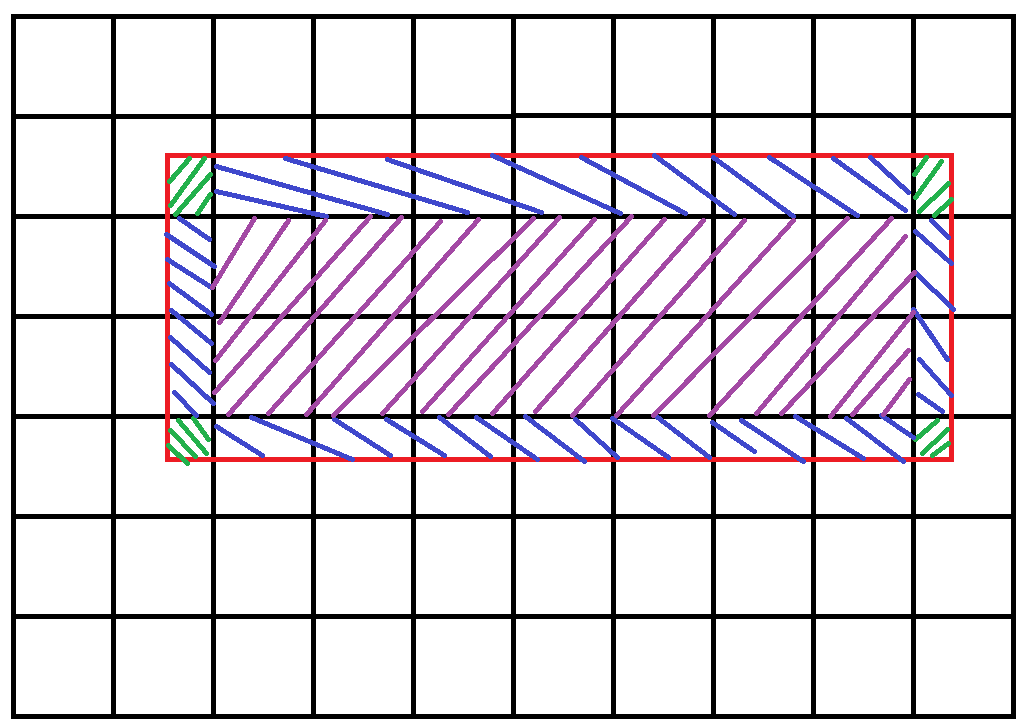
\includegraphics[width=\textwidth]{../figures/RMQ_query.png}
\caption{\label{fig:rmq_query}A typical 2D range query. Green is the corners, blue is the sides, and purple is the full blocks.}
\end{figure}

It consists of four corners, four sides, and an area consisting of several full blocks. We will answer the query for each of the nine parts separately and take the minimum of them.
A corner query will typically look as in Figure~\ref{fig:rmq_corner}. This type of query can trivially be answered in $\mathcal{O}(\max(\sqrt{n},\sqrt{m}))$ by taking the minimum of up to $\max(\sqrt{n},\sqrt{m})$ range queries each taking constant time.
\begin{figure}[htbp!]
    \centering
    \begin{subfigure}[b]{0.49\textwidth}
        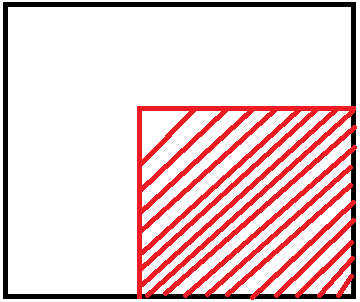
\includegraphics[width=\textwidth]{../figures/RMQ_corner.png}
        \caption{A typical corner query for 2D RMQ}
        \label{fig:rmq_corner}
    \end{subfigure}
    \begin{subfigure}[b]{0.49\textwidth}
        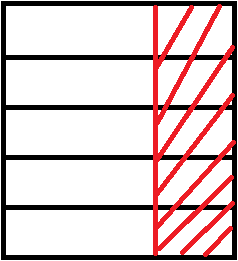
\includegraphics[width=\textwidth]{../figures/RMQ_side.png}
        \caption{A side in the 2D RMQ query}
        \label{fig:rmq_side}
    \end{subfigure}
\end{figure}

A side query may look as in Figure~\ref{fig:rmq_side}. The side query may be answered by a single range query to each block on the side since the elements queried is next to each other in the 1D RMQ structure. We know that we have at most $\Theta(\max(\sqrt{m},\sqrt{n}))$ such queries to make which gives a total time of $\mathcal{O}(\max(\sqrt{m},\sqrt{n}))$ for each side.
Now we only need to handle the full blocks. Since we have built a Cartesian tree on top of the blocks we will be able to answer such queries in a similar way to the other types. We simply make up to $\Theta(\max(\sqrt{m},\sqrt{n}))$ range queries and take the minimum of those.

This solution will require $\mathcal{O}(N)$ space since we use $\sqrt{nm} \cdot \sqrt{nm} = N$ for the $N$ blocks and $N$ space for the Cartesian tree on top of the blocks. We will be able to answer a query in $\mathcal{O}(\max(\sqrt{m},\sqrt{n}))$.

Dividing in blocks of size $\log n \times \log m$ will give a solution with $\left\langle \mathcal{O}(N\log N),\ \mathcal{O}(\log N)\right\rangle$ space and time.

It is shown by Brodal et al\cite{algorithmica12min} that the 2D RMQ can be solved with $\mathcal{O}(N)$ space and $\mathcal{O}(1)$ query time with an additional $\mathcal{O}(N)$ bits.


\chapter{Nearest common ancestors under leaf insertions and deletions}
\label{chp:LCA}
\subsection{Problem description}
\textit{Describe a data structure to maintain a tree $T$ under the insertion and deletion of leafs (to insert a new leaf we are given a pointer to the parent node), while supporting nearest common ancestor queries of two arbitrary nodes in $T$. State the update and query time of your data structure.}

\textit{What are the best update and query bounds you can achieve?}

\subsection{Solution}
Might not be magic!

\chapter{In-place merging}
\label{chp:inplace}
\subsection{Problem description}
\textit{Describe an algorithm that given an array containing $m+n$ elements $x_1x_2\dots x_m y_1y_2\dots y_n$, where $x_1\leq x_2\leq \dots \leq x_m$ and $y_1\leq y_2\leq \dots \leq y_n$, inplace merges the two sorted sequences. State the running time of your algorithm.}

\textit{What is the best running time you can achieve?}

\subsection{Introduction}
Merging is the process of combining two pre-sorted lists to create a single sorted list. The natural way to merge two lists is to repeatedly compare the smallest elements from both lists and then output the smallest of the two. This is repeated until both lists are exhausted. This process requires $m+n-1$ comparisons and $m+n$ data moves. A merge is called stable if it preserves the order of the elements in the respective lists.

In this exercise we will look at merging two sorted lists in-place. A merge algorithm is said to be in-place if it uses no more than $\mathcal{O}(1)$ extra memory.

A solution to the problem of in-place merging two pre-sorted lists will be presented in the next section. This solution is not stable but is shown to be optimal up to the values of constants of proportionality in the space-time bounds. The solution was first presented by Kronrod in 1969\cite{Kronrod}.

\subsection{Kronrod}
Initially we chop up the two pre-sorted lists into blocks of size $k$, i.e. $k$ is the number of elements in each block. We set $k =\sqrt{m+n}$. The last element in each block is selected. We call this element the mark of each block. The blocks are then rearranged in sorted order according to the mark of each block into a list $L$ of length $m+n$. We can now conclude that each element is at most $k$ positions away from their final position in the merged array.

We now use the last two blocks in $L$ as a temporary output location for our merge operation. This means that the last two blocks become unsorted. When the temporary buffer becomes full, i.e. we have merged two blocks fully, we swap the two merged blocks that reside in the temporary buffer with the old unmerged blocks such that the merged blocks find their correct position in the list. We do this for all blocks until we reach the final two blocks. These blocks are the unsorted temporary buffer. The two buffers can be sorted using a selection sort in time $\mathcal{O}(2\cdot\left(\sqrt{m+n}\right)^2) = \mathcal{O}(m+n)$.

\subsection{Time complexity}
The initial rearrangement is a sorting of the marks. We have $\mathcal{O}(\sqrt{m+n})$ such marks and running an insertion sort on these element will run in $\mathcal{O}( (\sqrt{m+n})^2) = \mathcal{O}(m+n)$ time.

Merging two blocks consumes one comparison per element resulting in $m+n - 2\sqrt{m+n} = \mathcal{O}(m+n)$ comparisons.

Finally the last two blocks which makes up the temporary buffer are sorted using selection sort in time $\mathcal{O}(2\cdot\left(\sqrt{m+n}\right)^2) = \mathcal{O}(m+n)$.

In total we do $3\cdot\mathcal{O}(m+n) = \mathcal{O}(m+n)$ comparisons giving a linear time algorithm in the size of the input which is asymptotically optimal.

%We can also argue about the number of data moves. Block rearrangement consumes 

\chapter{Prefix counting}
\label{chp:prefix}
\subsection{Problem description}
\textit{Let $A$ be an array of size $n$, where each $A\left[i\right]$ is either $0$ or $1$. Describe a data structure that supports updating an entry of $A$ to either $0$ or $1$, and the query $sum_2\left(i\right)$ that returns $\left(A\left[1\right]+A\left[2\right]+\dots+A\left[i\right]\right)\mod 2$, i.e. decides if the sum of the first $i$ entries of $A$ is odd or even.}

\textit{What is the best query time and update time you can achieve? A lower bound of $\Omega(\log n/\log\log n)$ is known for the operations on the RAM.}

\textit{Optional: Generalize the construction to return the sum $A[1]+A[2]+\dots+A[i]$, i.e. the number of entries equal one among the first $i$ entries.}

\subsection{Solution}
We construct a tree of height $\Theta(\nicefrac{\log n}{\log\log n})$ by having a fanout of size $\log n$. The leafs of the tree is the array elements, and internal nodes store the parity of the subtree. Furthermore we build a table of size $2^{\log n} = n$ storing every combination of parity for blocks of length $\log n$. This table will allow us to calculate the parity of a block in constant time by a single table lookup.

We are now ready to describe how to update and query the structure:
\begin{itemize}
	\item{$Update(i, x)$ - Traverse down the tree to leaf $i$ and update the value. If the value changes then recursively change the parity of all the internal nodes up the tree.}
	\item{$Query(i)$ - Figure~\ref{fig:pre_query} shows a typical query. To answer this query we traverse down the tree to $j$. Here we answer the subquery up to $k$ by a table lookup. This answer is combined with a table lookup for the missing partial block.}
\end{itemize}

\begin{figure}
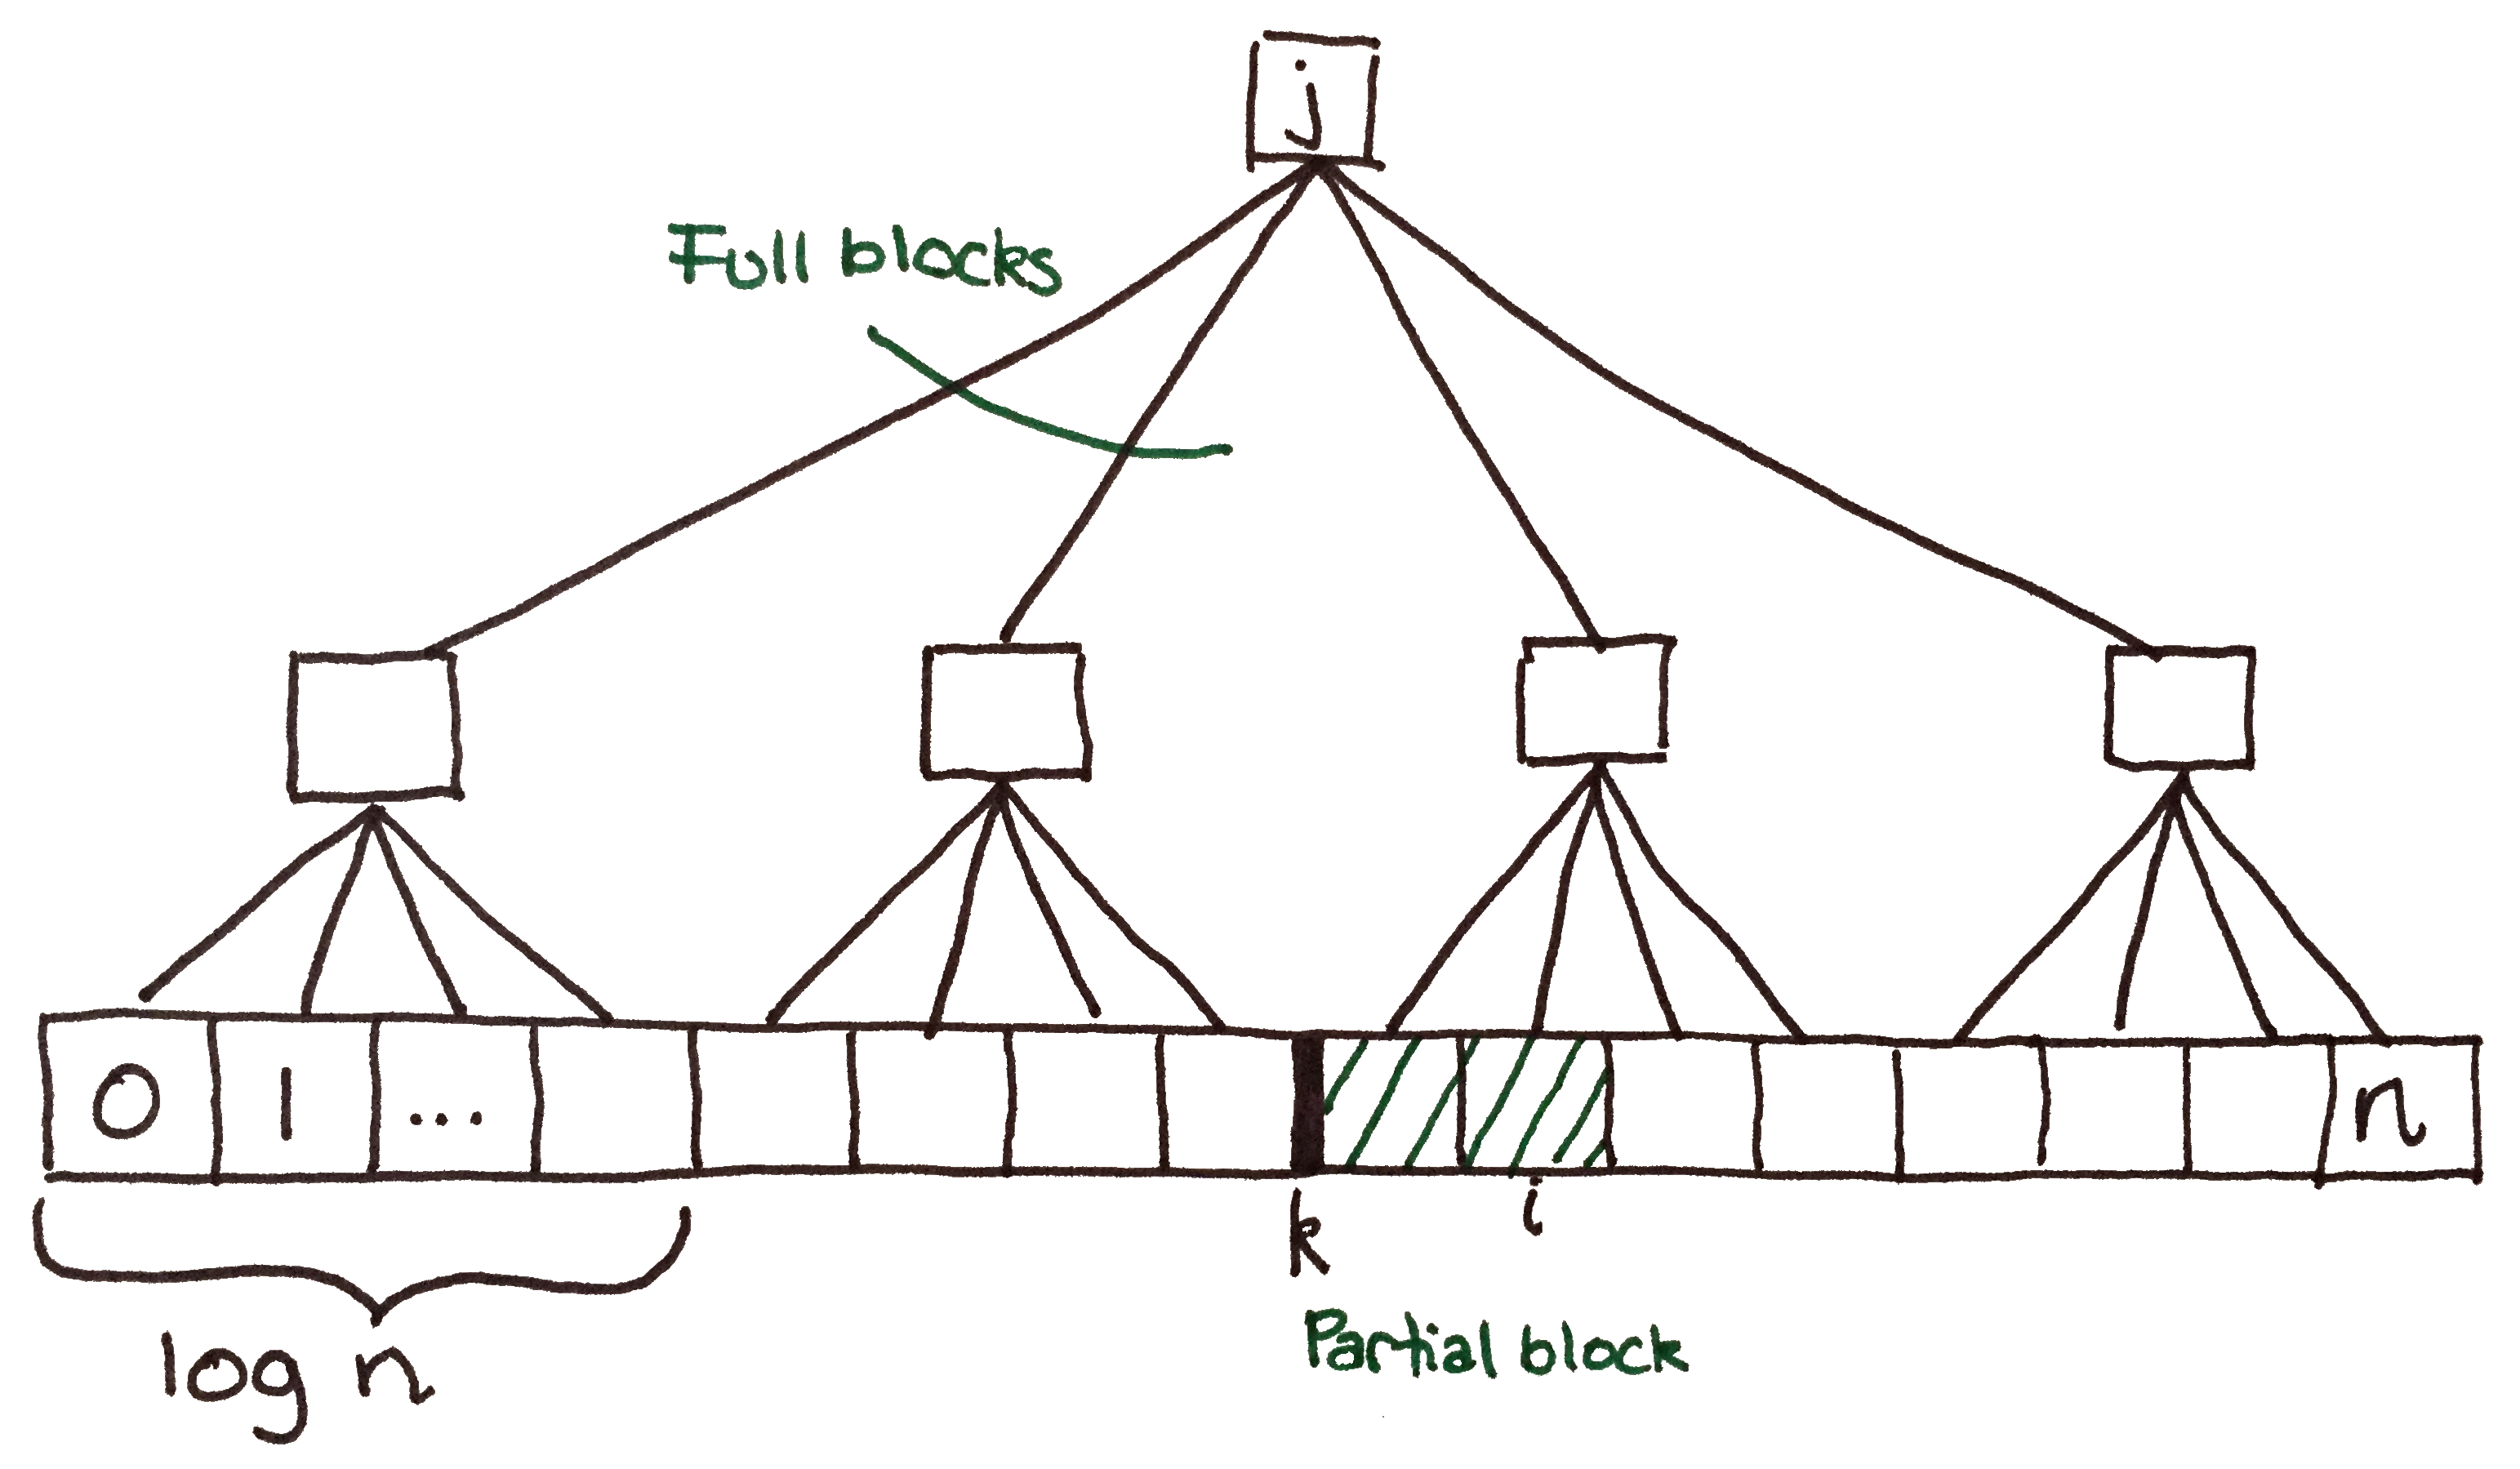
\includegraphics[width=\textwidth]{../figures/pre_query.png}
\caption{\label{fig:pre_query}A typical prefix query}
\end{figure}

\subsection{Complexity}
Update will simply traverse the tree up and down and update a single value in each step. This will give a complexity equal the height of the tree, i.e. a complexity of $\mathcal{O}(\nicefrac{\log n}{\log\log n})$.

A query is answered by traversing down the tree and doing two table lookups. Once again this gives a complexity equal the height of the tree, $\mathcal{O}(\nicefrac{\log n}{\log\log n})$.

These bounds are optimal!

\bibliography{references}

\end{document}


